\section{Analisi dei requisiti}
Come descritto nell'introduzione, abbiamo progettato un applicativo per la gestione e organizzazione dell'utilizzo di navette fornite dall'università per dare la possibilità a studenti di fare spostamenti tra quelle sedi universitarie che non sono dotate di un trasporto pubblico adatto.
Abbiamo individuato come attori principali i seguenti:
\begin{itemize}
    \item \textbf{Studente}: utente a cui è rivolto principalmente l'applicativo; 
    \item \textbf{Admin}:  utente autorizzato alla gestione delle risorse e degli utenti
\end{itemize}
Gli studenti avranno la possibilità di creare un profilo nel quale dovranno inserire i propri dati, e successivamente potranno aggiungersi a viaggi già esistenti o crearne nuovi, indicando data, orario, sede di partenza e sede di arrivo; devono poter modificare o cancellare le proprie prenotazioni, e le proprie credenziali.
\\L'admin invece deve avere totale controllo delle risorse disponibili, potendo aggiungere o eliminare navette in caso di guasti o di nuove disponibilità, e cancellare o modificare i viaggi. Deve avere anche la possibilità di gestire i profili utenti, revocare la possibilità di guida oppure rimuovere profili.
\subsection{Use Case Diagrams}
I seguenti sono gli Use Case diagrams trovati contenenti i casi d'uso più principali riguardanti gli attori \textit{Student} (vedi fig \ref{fig:ucSTU}), e \textit{Admin} (vedi fig.\ref{fig:ucADM}):
\begin{figure}[H]
    \centering
    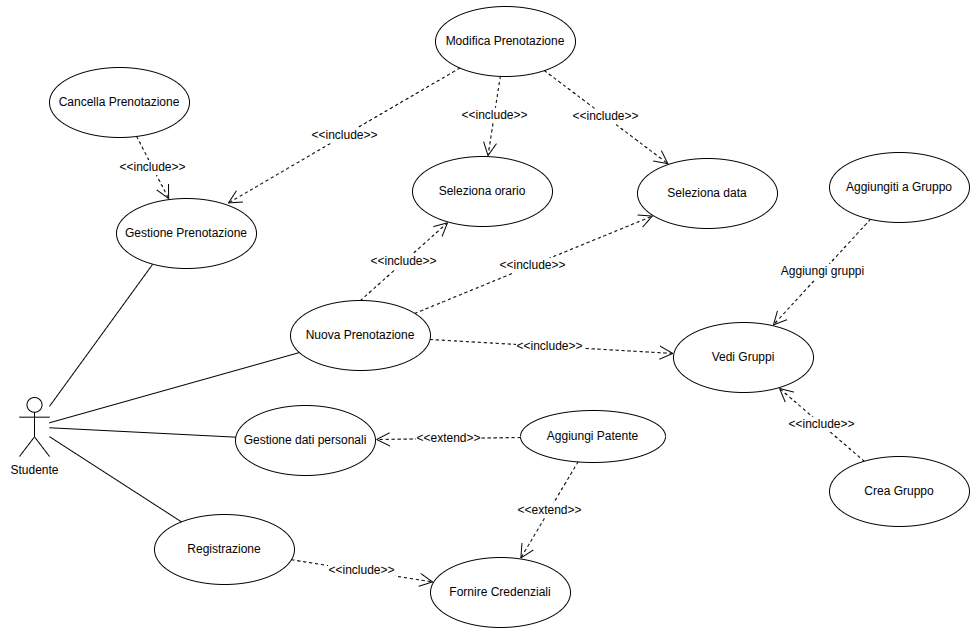
\includegraphics[width=1.2\linewidth]{Images/Student UC.png}
    \caption{Use Case diagram per Studente}
    \label{fig:ucSTU}

    \vspace{0.5cm}

    \centering
    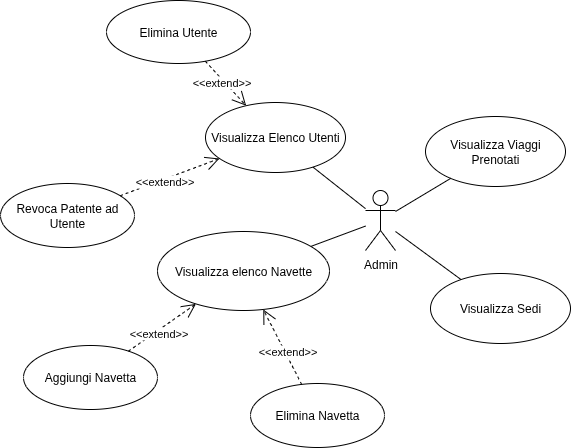
\includegraphics[width=1\linewidth]{Images/Admin UC.png}
    \caption{Use Case diagram per Admin}
    \label{fig:ucADM}
\end{figure}
\subsection{Use Case Template}\label{subsec:usecaseTemplate}
Di seguito sono riportati gli use case template per i principali casi d'uso del progetto; ognuno di questi descrive in modo strutturato alcune funzionalità del sistema.


% Macro per i casi d'uso

\newcommand{\UseCase}[9]{%
\begin{table}[H]
    \centering
    \small
    \begin{tabularx}{\textwidth}{lX}
        \toprule
        \rowcolor{grey!20} \textbf{Use Case \##1} & \textbf{#2} \\
        \midrule
        \rowcolor{white} \textbf{Brief Description} & #3 \\
        \rowcolor{blue!10} \textbf{Level} & #4 \\
        \rowcolor{white} \textbf{Actors} & #5 \\
        \rowcolor{blue!10} \textbf{Pre-conditions} & #6 \\
        \rowcolor{white} \textbf{Basic Flow} & #7 \\
        \rowcolor{blue!10} \textbf{Alternative Flows} & #8 \\
        \rowcolor{white} \textbf{Post-conditions} & #9 \\
        \bottomrule
    \end{tabularx}
\end{table}
}
% Use Case 1
\UseCase 
{1}
{Studente - Registrazione}
{Lo studente crea un nuovo account sull'applicazione.}
{User Goal}
{Studente}
{\begin{description}[nosep]
    \item[-] Studente non è ancora registrato
    \item[-] Si trova nella schermata di login/sign up
\end{description}}
{\begin{description}[nosep]
    \item[1.] Utente seleziona "Registrati"
    \item[2.] Sistema mostra il form di registrazione (vedi mockup fig. \ref{mockUp:registerMockup})
    \item[3.] L'utente inserisce i dati richiesti
    \item[4.] Conferma la registrazione
    \item[5.] Viene fatto il login automatico
\end{description}}
{\begin{description}[nosep]
    \item[4a.] Dati non validi → sistema mostra errore
\end{description}}
{L'account dello studente è creato e salvato nel database}
\label{uc:uc1}

% Use Case 2
\UseCase
{2}
{Visualizza viaggi disponibili}
{Lo studente cerca viaggi già programmati per una specifica tratta e fascia oraria.}
{User Goal}
{Studente}
{Lo studente ha effettuato l’accesso all’applicazione e si trova nella schermata principale.}
{\begin{description}[nosep]
    \item[1.] Dalla pagina principale, lo studente sceglie l'opzione per visualizzare i viaggi disponibili (vedi mockup fig.\ref{mockUp:viewTrips})
    \item[2.] Lo studente inserisce la sedi di partenza e arrivo, il giorno e la fascia oraria
    \item[3.] Il sistema mostra i viaggi compatibili
\end{description}}
{\begin{description}[nosep]
    \item[3a.] Nessun viaggio compatibile con i criteri di ricerca → sistema mostra opzioni per creare nuovo viaggio (vedi mockup fig. \ref{mockUp:createTrip})
\end{description}}
{L'utente visualizza la lista dei viaggi disponibili per i criteri scelti} 
% Use Case 3
\UseCase
{3}
{Aggiungiti a Viaggio Esistente}
{Lo studente si unisce a un viaggio esistente come passeggero.}
{User Goal}
{Studente}
{Lo studente sta visualizzando la lista dei viaggi (vedi mockup \ref{mockUp:viewTrips}).}
{\begin{description}[nosep]
    \item[1.] Lo studente seleziona un viaggio
    \item[2.] Premendo "Aggiungiti", il sistema verifica disponibilità
    \item[3.] Il sistema associa la prenotazione al viaggio
    \item[4.] Sistema mostra la conferma della prenotazione
\end{description}}
{\begin{description}[nosep]
    \item[2a.] Viaggio pieno → sistema mostra errore
\end{description}}
{Lo studente è stato aggiunto come passeggero al viaggio scelto}
\label{uc:uc3}
% Use Case 4
\UseCase
{4}
{Crea Nuovo Viaggio}
{Lo studente crea un nuovo viaggio proponendosi come guidatore.}
{User Goal}
{Studente (Guidatore)}
{\begin{description}[nosep]
    \item[-] UC-2 non ha prodotto risultati
    \item[-] Studente è registrato come Guidatore
    \item[-] Ci sono dei veicoli disponibili
\end{description}}
{\begin{description}[nosep]
    \item[1.] Dopo una ricerca negativa, sistema mostra "Crea Nuovo Viaggio"
    \item[2.] Studente seleziona l'opzione e conferma la creazione
    \item[3.] Sistema crea nuovo Trip con studente come Driver
    \item[4.] Sistema mostra conferma creazione
\end{description}}
{\begin{description}[nosep]
    \item[3a.] Viaggio identico creato da altri → sistema annulla e propone di unirsi
\end{description}}
{Un nuovo viaggio è stato creato con lo studente come guidatore}
\label{uc:uc4}
% Use Case 5
\UseCase
{5}
{Admin - Elimina Utente}
{L’amministratore elimina un account utente.}
{User Goal}
{Admin}
{L’utente è registrato nel sistema.}
{\begin{description}[nosep]
    \item[1.] Admin accede alla gestione utenti
    \item[2.] Cerca un utente per nome, matricola o email
    \item[3.] Seleziona l’utente da eliminare
    \item[4.] Conferma l’eliminazione
    \item[5.] L'utente viene eliminato dal sistema
\end{description}}
{\begin{description}[nosep]
    \item[3a.] L’utente ha prenotazioni future o è assegnato come guidatore in un viaggio → sistema richiede conferma aggiuntiva
\end{description}}
{L’utente è rimosso dal sistema, incluse eventuali prenotazioni}
\label{uc:uc5}
% Use Case 6
\UseCase
{6}
{Admin - Aggiungi Navetta}
{L’admin registra una nuova navetta nel sistema.}
{Function}
{Admin}
{L’admin è autenticato e c'è un nuovo mezzo.}
{\begin{description}[nosep]
    \item[1.] Admin accede alla sezione "gestione navette"
    \item[2.] Sistema mostra il form per inserire i dati del veicolo
    \item[3.] Admin inserisce i dati della nuova navetta (posti, targa, ecc.)
    \item[4.] Conferma l’inserimento
    \item[5.] Viene aggiornata la lista dei veicoli
\end{description}}
{\begin{description}[nosep]
    \item[2a.] Dati non validi → sistema mostra errore
    \item[3a.] La navetta è già presente → impedisce duplicazione
\end{description}}
{La navetta è disponibile per l’assegnazione ai gruppi}
\label{uc:uc6}
\subsection{Page Navigation Diagram}\label{subsec:PageNavigation}
Nel seguente diagramma sono riportate le possibili azioni che un utente può compiere, mostrando i modi con il quale si può navigare tra le pagine.
\begin{figure}[H]
    \centering
    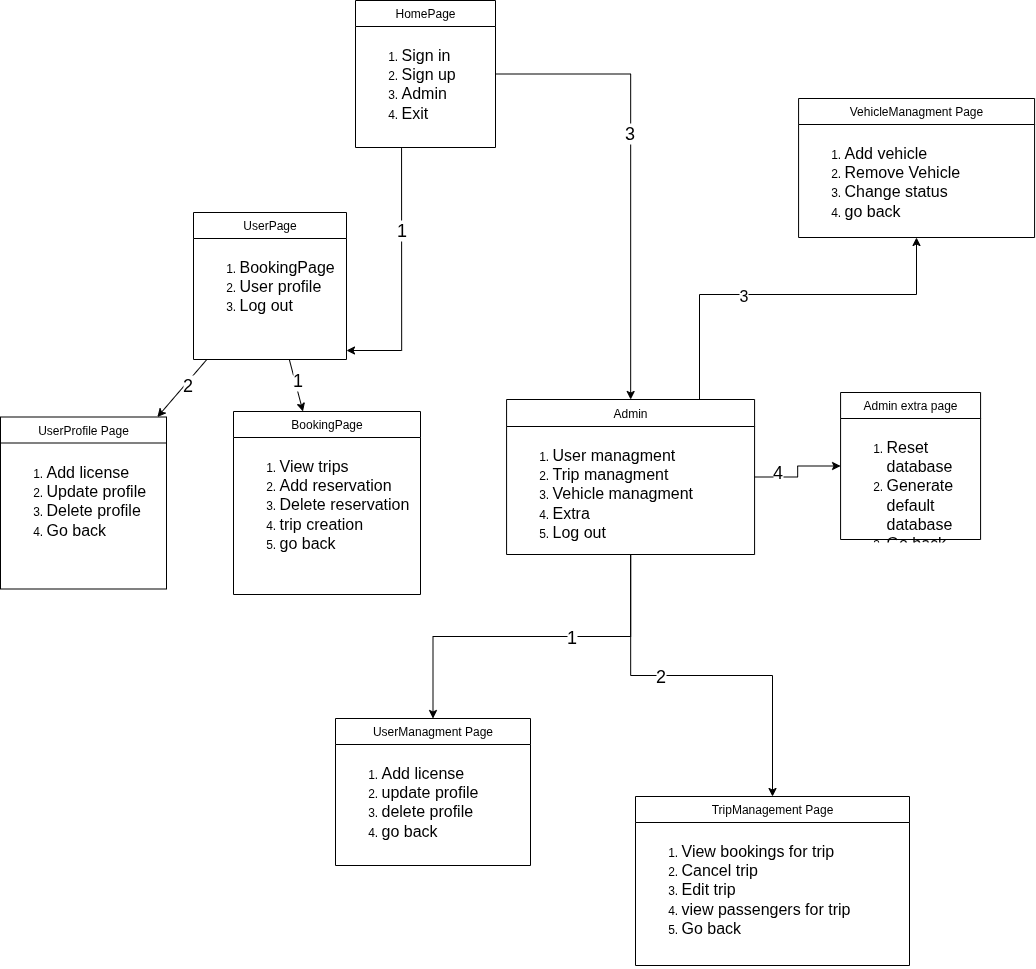
\includegraphics[width = 1.25\linewidth]{Images/PageNavigation_diag.png}
    \caption{Page Navigation Diagram}
    \label{fig:PageNavdiag}
\end{figure}
\subsection{Mockup}
Di seguito presentiamo alcune rappresentazioni grafiche di una possibile implementazione dell'interfaccia utente del sistema. Le immagini sono state realizzate con Figma, uno strumento dedicato alla progettazione di interfacce grafiche. La scelta di proporre mockup per dispositivi mobili è motivata dall'ipotesi che la maggior parte degli utenti accederà al servizio tramite smartphone.
\begin{figure}[H]
    \centering
    \begin{minipage}{0.45\textwidth}
        \centering
        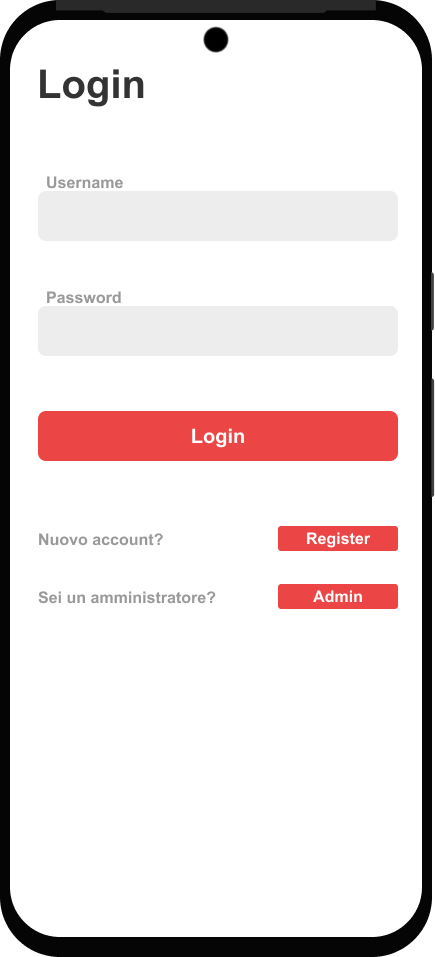
\includegraphics[width=\linewidth]{Images/Login Page.png}
        \caption{Schermata di login}
        \label{mockUp:loginMockup}
    \end{minipage}%
    \hfill
    \begin{minipage}{0.45\textwidth}
        \centering
        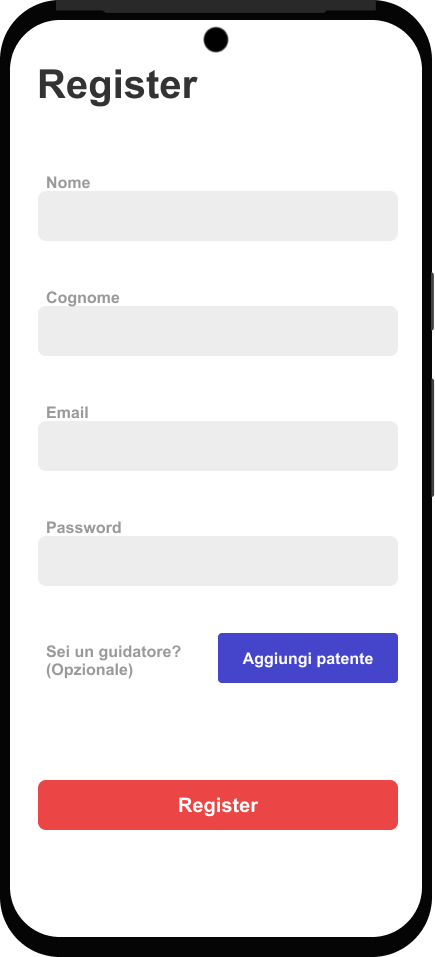
\includegraphics[width=\linewidth]{Images/Register page.png}
        \caption{Schermata di registrazione}
        \label{mockUp:registerMockup}
    \end{minipage}
\end{figure}


\begin{figure}[H]
    \centering
    \begin{minipage}{0.45\textwidth}
        \centering
        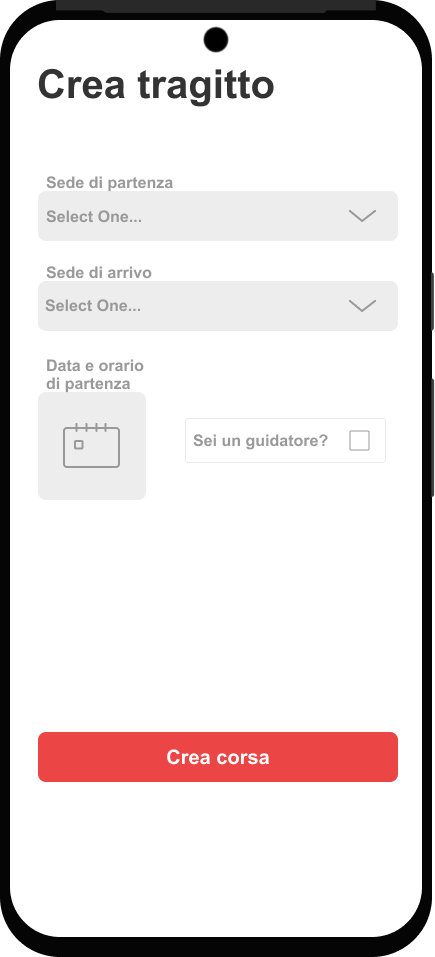
\includegraphics[width=\linewidth]{Images/Crea tragitto.png}
        \caption{Schermata di creazione tragitto}
        \label{mockUp:createTrip}
    \end{minipage}%
    \hfill
    \begin{minipage}{0.45\textwidth}
        \centering
        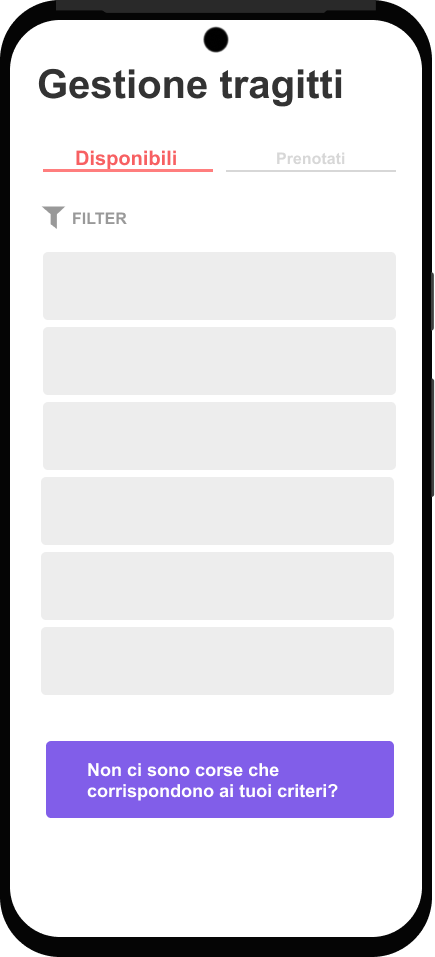
\includegraphics[width=\linewidth]{Images/Tragitti disponibili.png}
        \caption{Schermata di visualizzazione dei viaggi}
        \label{mockUp:viewTrips}
    \end{minipage}
\end{figure}
\section{Class Diagram}
Vista la progettazione a tre livelli, di seguito sono riportati i diagrammi delle classi per ciascuno dei modelli.
Nella figura \ref{fig:pkdep} è possibile osservare le dipendenze tra i vari package del sistema.
\begin{figure}
    \centering
    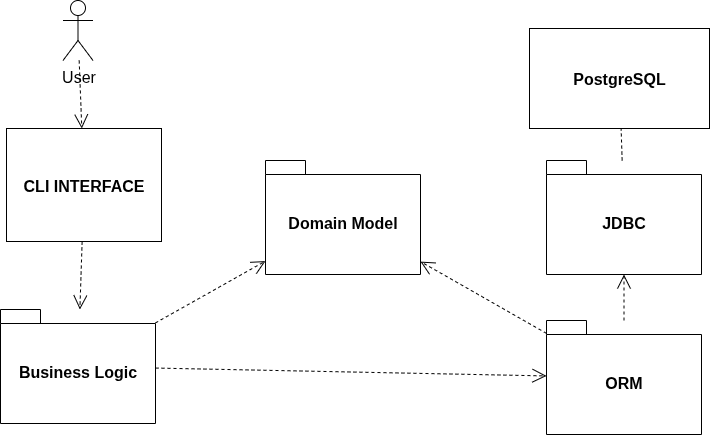
\includegraphics[width=1\linewidth]{Images/PkgDeps.png}
    \caption{Package Dependency Diagram}
    \label{fig:pkdep}
\end{figure}
\subsection{Domain Model}\label{subsec:DM}
Il Domain Model ha il compito di definire le entità concettuali fondamentali del dominio dell'applicazione; le sue classi rappresentano i concetti del "\textit{mondo reale}", infatti le istanze saranno utilizzate negli altri layer dell'applicazione per eseguire elaborazioni sui dati senza richiedere un accesso diretto al database; solitamente sono implementate come \textit{POJO} (\textit{Plain Old Java Object}), non avendo nessun tipo di metodi oltre a getters e setters.
Le entità principali che abbiamo individuato sono le seguenti:
\begin{itemize}
    \item \textbf{User}: è la classe che rappresenta gli utenti; abbiamo deciso di distinguere studenti ed admin tramite l'uso di un attributo \texttt{UserRole role} dato che in questo contesto condividono  tutti gli altri attributi, ma nello strato di business avranno diversi privilegi operativi
    \item \textbf{Trip}: rappresenta un viaggio organizzato incapsulando tutte le informazioni sul viaggio tra cui: origine, destinazione, data, orario, guidatore assegnato e veicolo
    \item \textbf{Booking}: modella le prenotazioni fatte dagli studenti per i viaggi; in questa abbiamo deciso di non mettere data e orario perché sarebbe stata una duplicazione essendo già presenti nell'attributo di tipo Trip
    \item \textbf{Location}: modella le sedi universitarie tra le quali gli studenti possono spostarsi
    \item \textbf{Vehicle}: rappresenta le navette che verranno usate nei viaggi
\end{itemize}
Nel seguente diagramma di classe vengono visualizzate le relazioni di composizione tra le classi.
\begin{figure}[H]
    \centering
    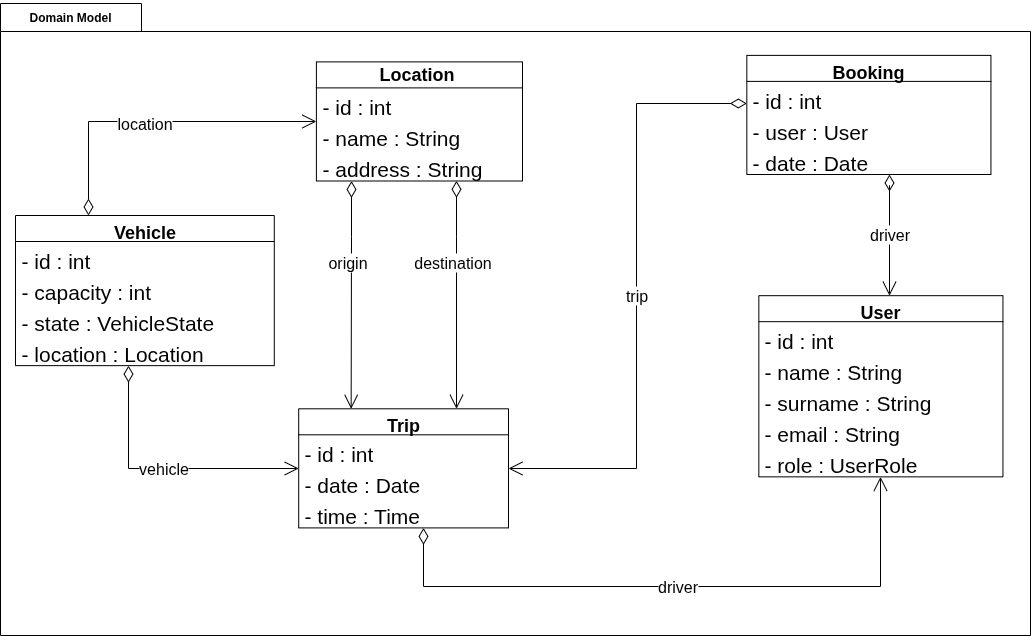
\includegraphics[width=1.2\linewidth]{Images/DomainModel_diag.png}
    \caption{Domain Model class diagram}
    \label{fig:DMdiag}
\end{figure}
\subsection{ORM}\label{subsec:ORM}
Questo livello ha il compito di gestire l'interazione con il database scelto; viene implementato il design pattern DAO (\textit{Data Access Object}) fornendo un livello di astrazione utile per separare la logica di accesso ai dati nel database dalle operazioni di controllo e le entità del dominio applicativo.
Questo approccio consente di riutilizzare la stessa logica di business su diversi database, modificando unicamente l’implementazione dei DAO e riducendo così l’accoppiamento tra i livelli.\\
Nel livello ORM è presente un DAO per ciascuna entità del Domain Model, ognuno dei quali implementa le operazioni CRUD. Inoltre, una classe di utilità denominata ConnectionManager centralizza la gestione della connessione al database, semplificando eventuali modifiche di configurazione senza impattare gli altri componenti.
Di seguito viene riportato il diagramma delle classi
\begin{figure}[H]
    \centering
    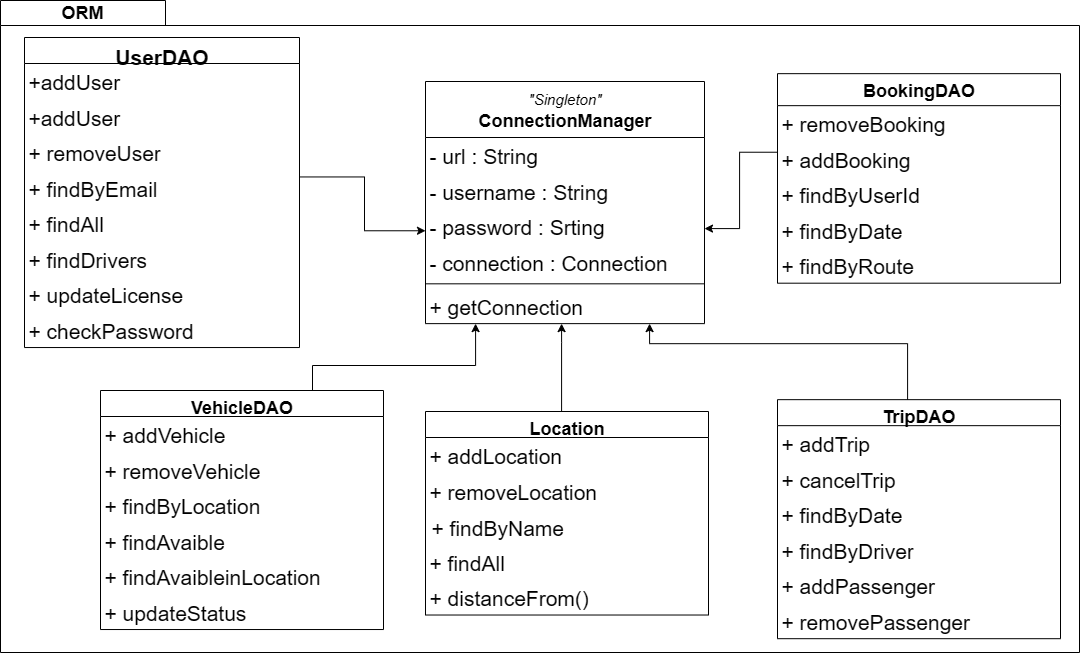
\includegraphics[width=1.1\linewidth]{Images/ORM_diag.png}
    \caption{ORM class diagram}
    \label{fig:ORMdiag}
\end{figure}
\subsection{Business Logic}\label{subsec:BL}
La Business Logic rappresenta la parte logica/operativa dell'applicazione; in questa vengono definite e implementate le regole di business e vengono coordinate tutte le possibili operazioni.\\
Questo strato fa quindi uso dei DAO per l'accesso ai dati persistenti e delle classi del Domain Model per l'elaborazione delle informazioni dei calcoli.
Ad ogni entità del Domain Model corrisponde un controller che ha il compito di gestire le operazioni principali che possono essere eseguite su quella entità; in più è presente una classe chiamata \texttt{AuthController} che si occupa della gestione dell'autenticazione e del controllo dei permessi degli utenti.
\begin{figure}[H]
    \centering
    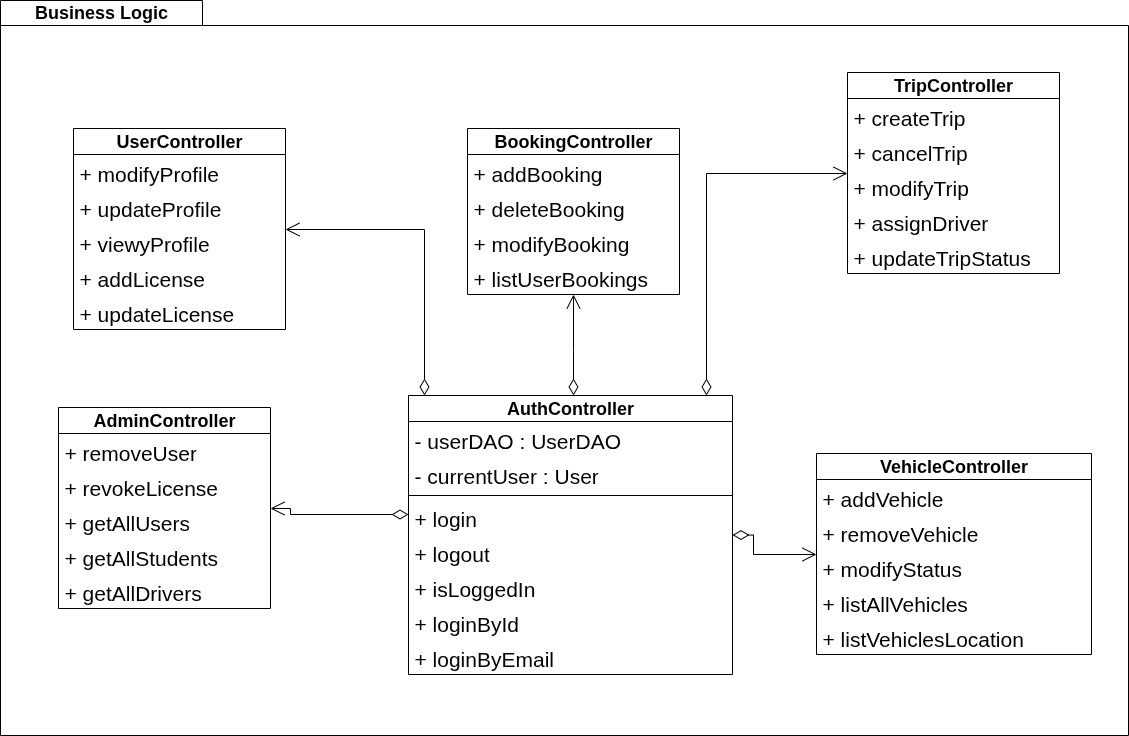
\includegraphics[width=1.1\linewidth]{Images/BusinessLogic_diag.png}
    \caption{Business Logic Diagram}
    \label{fig:BLdiag}
\end{figure}

\subsection{Diagramma ER e schema relazionale}\label{subsec:DB}
Per la progettazione del database abbiamo realizzato un diagramma ER (vedi fig. \ref{fig:ERdiag}),rappresentato in maniera più comprensibile (vedi fig. \ref{fig:ERraw}), e successivamente abbiamo costruito lo schema relazionale (vedi fig. \ref{fig:ERscheme}).
\begin{figure}[H]
    \centering
    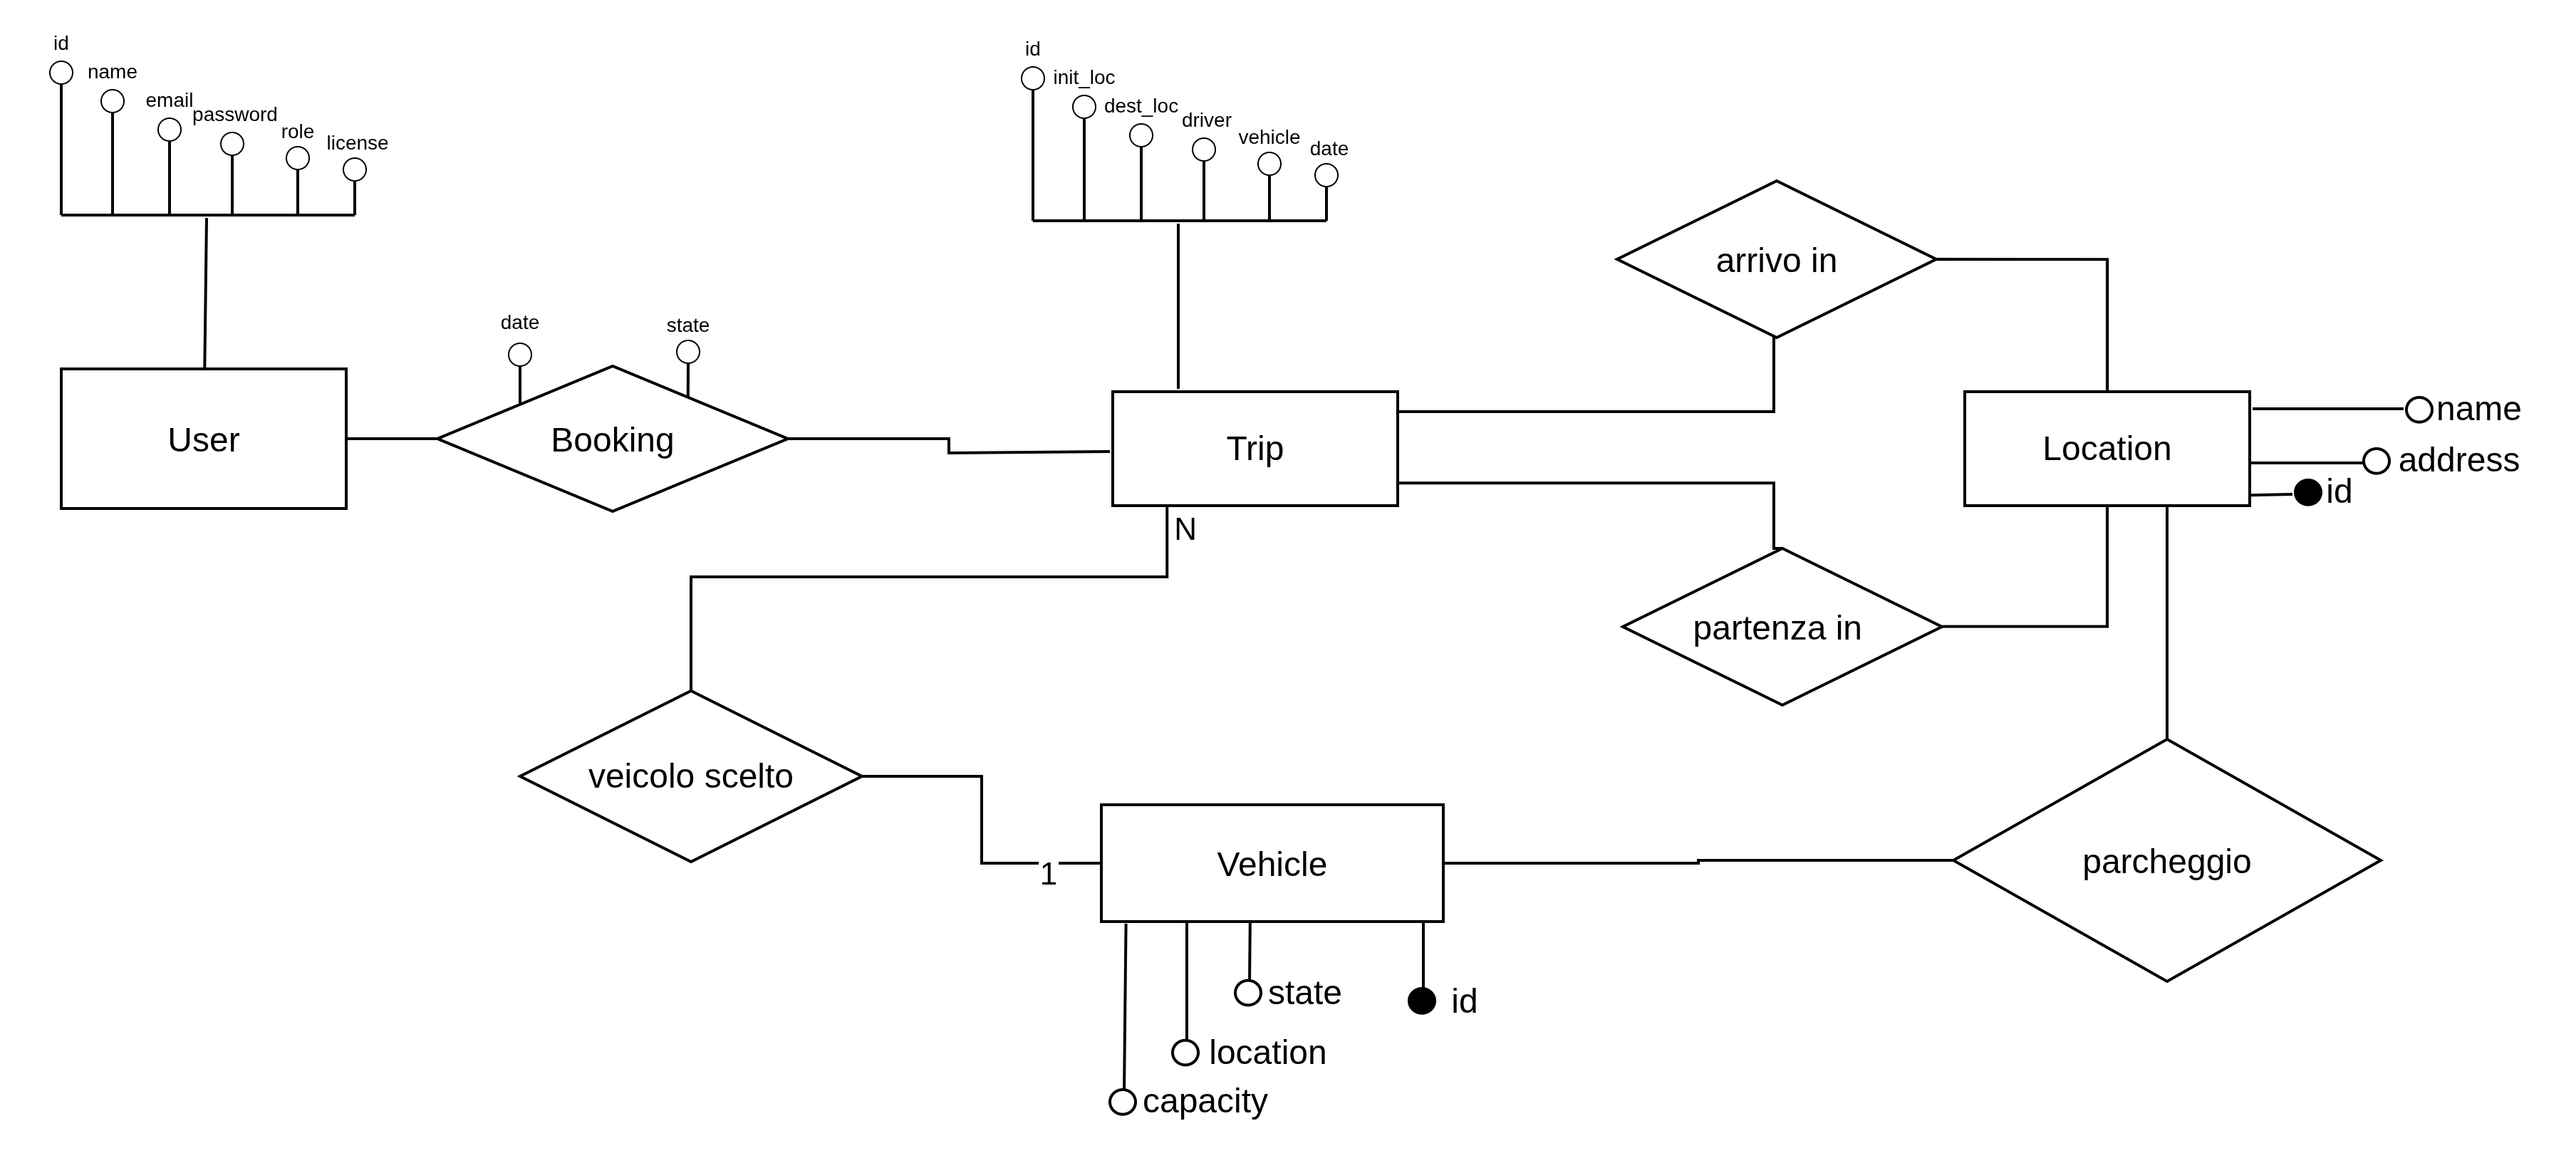
\includegraphics[width=1.1\linewidth]{Images/ER_diagram.png}
    \caption{ER diagram}
    \label{fig:ERdiag}
\end{figure}
\begin{figure}[H]
    \centering
    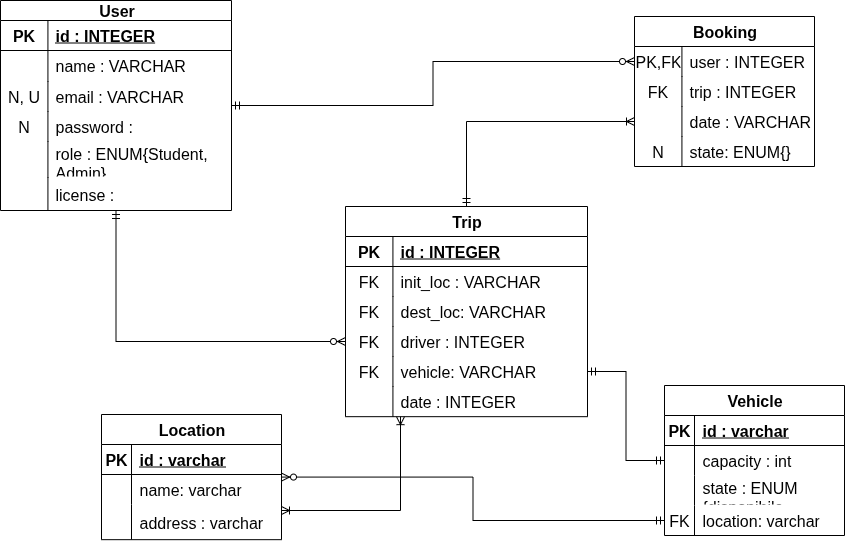
\includegraphics[width=1.2\linewidth]{Images/ERraw.png}
    \caption{ER diagram (rappresentazione semplificata)}
    \label{fig:ERraw}
\end{figure}
\begin{figure}[H]
    \centering
    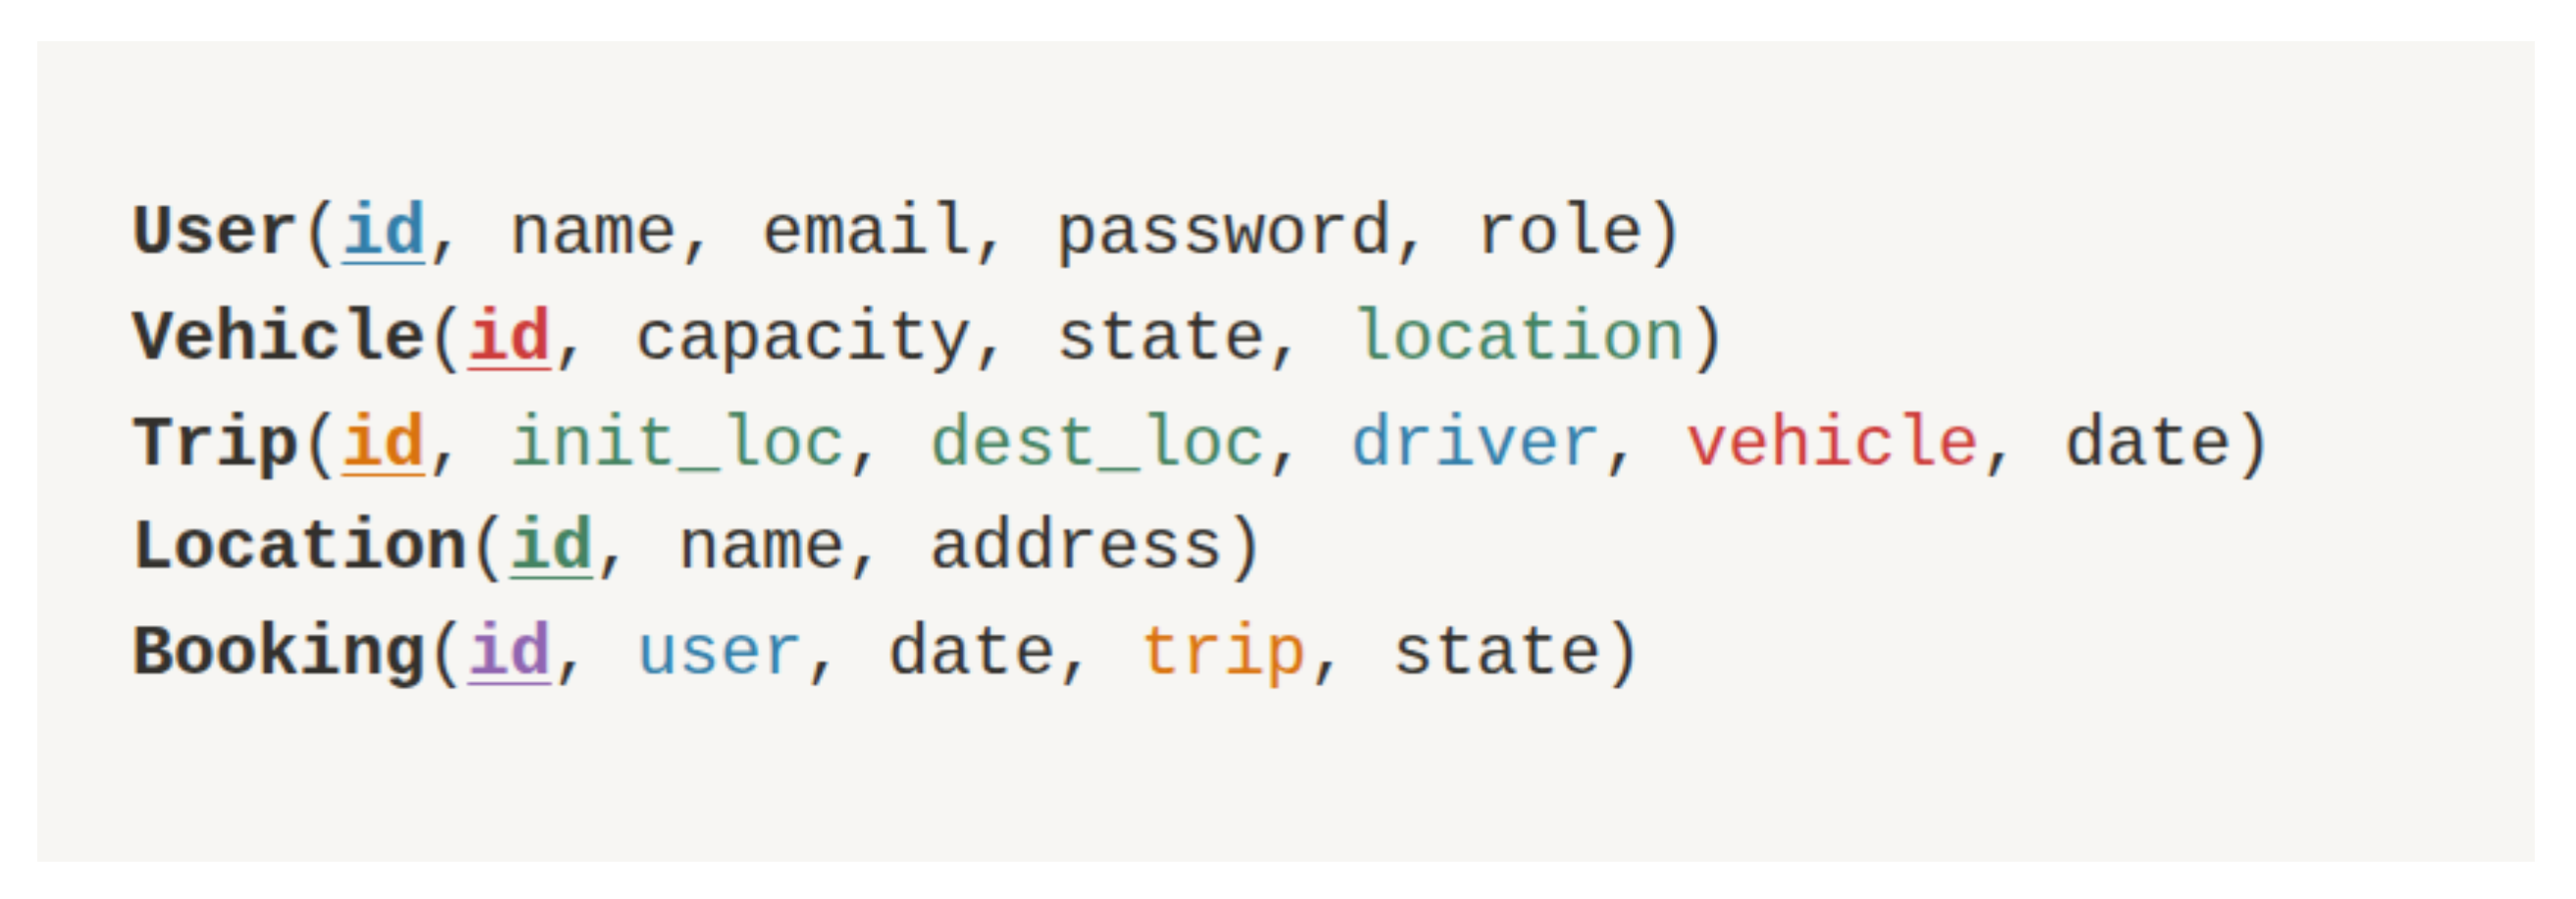
\includegraphics[width=0.8\linewidth]{Images/schema_relazionale.png}
    \caption{Schema relazionale}
    \label{fig:ERscheme}
\end{figure}
Come si può  vedere dai diagrammi, il modello ER è stato tradotto in tabelle relazionali, mantenendo le stesse entità e relazioni.